% System architecture. Compile: tectonic architecture.tex  (sized for a two-column figure*)
\documentclass[tikz,border=3pt]{standalone}
\usepackage{newtxtext,newtxmath}
\usetikzlibrary{arrows.meta,positioning,fit,backgrounds,calc}

\definecolor{ink}{HTML}{0B0B0B}
\definecolor{ink2}{HTML}{52514E}
\definecolor{rule}{HTML}{B9B8B2}
\definecolor{fillA}{HTML}{F3F2EE}
\definecolor{crypto}{HTML}{E8F1FB}
\definecolor{cryptoedge}{HTML}{2A78D6}
\definecolor{adv}{HTML}{E34948}

\tikzset{
  box/.style={draw=rule, fill=white, rounded corners=2pt, align=center,
              text width=5.0cm, minimum height=0.75cm, font=\footnotesize, inner sep=3pt},
  cbox/.style={box, draw=cryptoedge, fill=crypto, line width=0.6pt},
  small/.style={box, font=\scriptsize, minimum height=0.6cm, fill=fillA},
  party/.style={draw=ink2, rounded corners=4pt, inner sep=7pt, line width=0.6pt},
  flow/.style={-{Stealth[length=2mm]}, ink2, line width=0.6pt},
  msg/.style={-{Stealth[length=2.2mm]}, ink, line width=0.8pt},
  meter/.style={-{Stealth[length=1.6mm]}, ink2, densely dashed, line width=0.5pt},
  lbl/.style={font=\scriptsize, ink, fill=white, inner sep=1.5pt},
}

\begin{document}
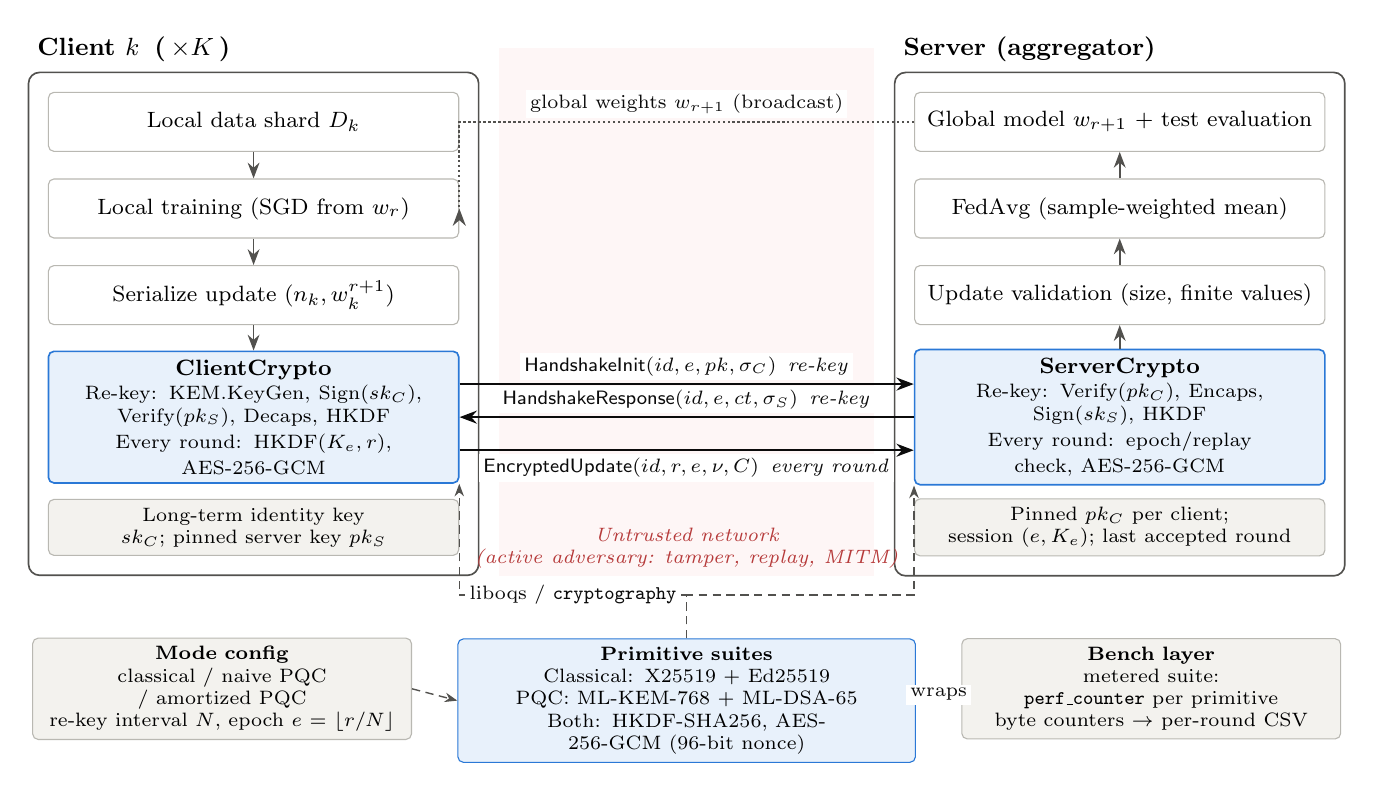
\begin{tikzpicture}[x=1cm, y=1cm]

% ---------------- Client k ----------------
\node[box]  (data)  at (3, 0)    {Local data shard $D_k$};
\node[box]  (train) at (3, -1.1) {Local training (SGD from $w_r$)};
\node[box]  (ser)   at (3, -2.2) {Serialize update $(n_k, w_k^{r+1})$};
\node[cbox, minimum height=1.45cm] (cc) at (3, -3.75)
  {\textbf{ClientCrypto}\\[1pt]
   \scriptsize Re-key: KEM.KeyGen, Sign$(sk_C)$,\\ \scriptsize Verify$(pk_S)$, Decaps, HKDF\\
   \scriptsize Every round: HKDF$(K_e, r)$, AES-256-GCM};
\node[small] (cid) at (3, -5.15) {Long-term identity key $sk_C$; pinned server key $pk_S$};
\draw[flow] (data) -- (train);
\draw[flow] (train) -- (ser);
\draw[flow] (ser) -- (cc);
\begin{scope}[on background layer]
  \node[party, fit=(data)(cid), label={[font=\small\bfseries, anchor=south west]north west:Client $k$ \,(\,$\times K$\,)}] (client) {};
\end{scope}

% ---------------- Server ----------------
\node[box]  (glob)  at (14, 0)    {Global model $w_{r+1}$ + test evaluation};
\node[box]  (avg)   at (14, -1.1) {FedAvg (sample-weighted mean)};
\node[box]  (val)   at (14, -2.2) {Update validation (size, finite values)};
\node[cbox, minimum height=1.45cm] (sc) at (14, -3.75)
  {\textbf{ServerCrypto}\\[1pt]
   \scriptsize Re-key: Verify$(pk_C)$, Encaps,\\ \scriptsize Sign$(sk_S)$, HKDF\\
   \scriptsize Every round: epoch/replay check, AES-256-GCM};
\node[small] (reg) at (14, -5.15) {Pinned $pk_C$ per client;\\ session $(e, K_e)$; last accepted round};
\draw[flow] (sc) -- (val);
\draw[flow] (val) -- (avg);
\draw[flow] (avg) -- (glob);
\begin{scope}[on background layer]
  \node[party, fit=(glob)(reg), label={[font=\small\bfseries, anchor=south west]north west:Server (aggregator)}] (server) {};
\end{scope}

% ---------------- Untrusted network ----------------
\coordinate (nl) at ($(client.east)+(0.25,0)$);
\coordinate (nr) at ($(server.west)+(-0.25,0)$);
\begin{scope}[on background layer]
  \fill[adv!5] ($(nl|-client.north)+(0,0.3)$) rectangle ($(nr|-client.south)$);
\end{scope}
\node[font=\scriptsize\itshape, adv!80!black, align=center] at ($(nl|-client.south)!0.5!(nr|-client.south)+(0,0.35)$)
  {Untrusted network\\(active adversary: tamper, replay, MITM)};

\draw[msg] ($(cc.east)+(0,0.42)$) -- node[lbl, above=1pt] {\textsf{HandshakeInit}$(id, e, pk, \sigma_C)$ \textit{\,re-key}}
           ($(sc.west)+(0,0.42)$);
\draw[msg] ($(sc.west)+(0,0)$) -- node[lbl, above=1pt] {\textsf{HandshakeResponse}$(id, e, ct, \sigma_S)$ \textit{\,re-key}}
           ($(cc.east)+(0,0)$);
\draw[msg] ($(cc.east)+(0,-0.42)$) -- node[lbl, below=1pt] {\textsf{EncryptedUpdate}$(id, r, e, \nu, C)$ \textit{\,every round}}
           ($(sc.west)+(0,-0.42)$);
\draw[msg, ink2, densely dotted] (glob.west) -- node[lbl, above=1pt] {global weights $w_{r+1}$ (broadcast)}
           (glob.west -| train.east) |- (train.east);

% ---------------- Shared layers ----------------
\node[small, text width=4.6cm, minimum height=1.1cm] (cfg) at (2.6, -7.2)
  {\textbf{Mode config}\\ classical / naive PQC / amortized PQC\\ re-key interval $N$, epoch $e=\lfloor r/N \rfloor$};
\node[small, text width=5.6cm, minimum height=1.1cm, fill=crypto, draw=cryptoedge] (suite) at (8.5, -7.35)
  {\textbf{Primitive suites}\\ Classical: X25519 + Ed25519\\ PQC: ML-KEM-768 + ML-DSA-65\\ Both: HKDF-SHA256, AES-256-GCM (96-bit nonce)};
\node[small, text width=4.6cm, minimum height=1.1cm] (bench) at (14.4, -7.2)
  {\textbf{Bench layer}\\ metered suite: \texttt{perf\_counter} per primitive\\ byte counters $\rightarrow$ per-round CSV};
\draw[meter] (suite.north) -- ++(0,0.55) -| (cc.south -| cid.east) node[pos=0.25, lbl] {liboqs / \texttt{cryptography}};
\draw[meter] (suite.north) -- ++(0,0.55) -| (sc.south -| reg.west);
\draw[meter] (cfg.east) -- (suite.west);
\draw[meter] (bench.west) -- (suite.east) node[midway, lbl] {wraps};

\end{tikzpicture}
\end{document}
